\documentclass[final,5p,times,twocolumn]{elsarticle}
\usepackage[T1]{fontenc}
\renewcommand{\ttdefault}{lmtt}
\usepackage{microtype,graphicx,booktabs,amsmath,amssymb,amsthm,array,tabularx,multirow}
\usepackage{xcolor,tikz,pgfplots,enumitem,xurl,placeins,balance}
\geometry{reset,a4paper,left=21mm,right=19mm,top=20mm,bottom=21mm,columnsep=6mm,footskip=10mm}
\usetikzlibrary{arrows.meta,positioning,calc,fit,backgrounds}
\pgfplotsset{compat=1.18}
\usepgfplotslibrary{groupplots}
\usepackage[hypertexnames=false,bookmarksnumbered=true]{hyperref}
\definecolor{target}{HTML}{355E7C}
\definecolor{draft}{HTML}{AB6B36}
\definecolor{qualified}{HTML}{39765C}
\definecolor{aux}{HTML}{68727B}
\definecolor{light}{HTML}{EDF2F5}
\hypersetup{colorlinks=true,linkcolor=target,citecolor=target,urlcolor=target,
pdfauthor={Chengzhan Li},pdftitle={HeteroSpec: Reference-Preserving Query Batching for Quantized Inference}}
\urlstyle{same}
\newcommand{\QB}{\mathrm{QB}}
\newcommand{\PQ}{\mathrm{PQ}}
\newcommand{\GS}{\mathrm{GS}}
\newcommand{\MQ}{\mathrm{MQ}}
\newcolumntype{Y}{>{\raggedright\arraybackslash}X}
\newtheorem{proposition}{Proposition}
\setlist{nosep,leftmargin=*}
\setlength{\emergencystretch}{2em}
\setlength{\tabcolsep}{4pt}
\renewcommand{\arraystretch}{1.15}
\renewcommand{\bibfont}{\small\raggedright}
\setlength{\textfloatsep}{13pt plus 3pt minus 2pt}
\setlength{\dbltextfloatsep}{14pt plus 3pt minus 2pt}
\renewcommand{\topfraction}{.9}
\renewcommand{\dbltopfraction}{.9}
\renewcommand{\textfraction}{.08}
\renewcommand{\floatpagefraction}{.72}
\renewcommand{\dblfloatpagefraction}{.72}
\setcounter{topnumber}{3}
\setcounter{dbltopnumber}{3}
\clubpenalty=8000
\widowpenalty=8000
\raggedbottom
\makeatletter
\def\ps@pprintTitle{\let\@oddhead\@empty\let\@evenhead\@empty\def\@oddfoot{\hfil\thepage\hfil}\let\@evenfoot\@oddfoot}
\makeatother
\pdfinfoomitdate=1
\pdftrailerid{}
\pdfsuppressptexinfo=15

\begin{document}
\begin{frontmatter}
\title{HeteroSpec: Reference-Preserving Query Batching for Quantized Inference}
\author{Chengzhan Li}
\address{University of Electronic Science and Technology of China, Chengdu, China\\[2pt]
{\normalfont\ttfamily\href{mailto:chengzhan.li@std.uestc.edu.cn}{chengzhan.li@std.uestc.edu.cn}}}
\begin{abstract}
Batching prompt or speculative-verification queries can change the output of an existing quantized deployment, even when their logical positions and causal masks are unchanged. We present a reference-preserving query-batching method that separates physical KV-prefix requirements from query-parallel work. It groups adjacent queries by the physical prefix required by the original scalar execution, retains the corresponding arithmetic paths, and lowers each group through paired query/mask views with shared KV storage. Controlled interventions on CUDA and Vulkan identify a common physical-prefix mechanism; Vulkan additionally requires preservation of the projection activation path. The repairs remove the known Llama divergence and preserve the original references on two independently selected panels of 24 previously unseen inputs, with exact committed full-vocabulary-vector correspondence. A distinct CUDA Qwen3-14B intervention preserves the reference by retaining scalar-path placement at a head-normalization/RoPE boundary. Complete-request measurements separate reference repair, layout cost and drafting. On the repaired Llama panels, QB reduces speculative cost relative to per-query attention by 2.45\% on CUDA and 4.95\% on Vulkan; the latter passes the predeclared practical screen. Drafting remains more expensive than the corresponding target-only paths. These results establish physical-prefix compatibility and arithmetic-path preservation as actionable constraints for retaining parallel execution against a deployed numerical reference.
\end{abstract}
\begin{keyword}
quantized inference \sep reference preservation \sep speculative decoding \sep attention batching \sep numerical execution
\end{keyword}
\end{frontmatter}
\section{Introduction}
An inference optimization can preserve the mathematical model and still change the behavior of a deployed numerical implementation. Quantized weights, finite-precision activations, physical cache extents and backend placement jointly determine the computation that produces a response. When a deployment's regression tests or downstream state are tied to an established numerical trace, replacing that trace with a different deterministic one does not satisfy the compatibility requirement. The practical question is therefore: \emph{which computations can be batched while preserving the existing reference?}

This question arises in both prompt processing and speculative decoding. Prompt tokens are known together; speculative decoding supplies several proposed continuation tokens for parallel verification~\cite{leviathan2023,chen2023}. Both expose independent query work inside a causal attention graph. Ordinary autoregressive continuation still generates one token at a time. The opportunity studied here is to retain the parallel work that is already available without changing how reference-sensitive operations are evaluated.

Existing approaches establish useful forms of determinism. Batch-invariant kernels stabilize per-token evaluation across batch sizes~\cite{thinkingmachines}. CoRun uses isolated prefill and fixed-shape decode~\cite{corun}. LLM-42 lets a fixed-shape verifier define a consistent execution, then repairs tokens and KV state~\cite{llm42}. Vosti connects canonical state to relational kernel contracts~\cite{vosti,vosticontract}. Our target is compatibility with a reference chosen before the optimization: the original quantized model bytes, numerical runtime and scalar execution recipe remain fixed.

Global serialization satisfies a simple execution constraint but removes batching from projections and feed-forward layers as well as attention. A more local approach evaluates attention separately for each query (PQ), leaving surrounding computation batched. Query-to-batch attention (QB) expresses this local organization through paired Q/mask views and shared K/V storage. However, agreement between PQ and QB is not sufficient: both can inherit a physical KV extent that differs from the scalar reference.

The decisive example is a four-query Llama verification crossing a padding boundary. The scalar executions use physical key extents $[768,768,768,1024]$, while the original batch uses $1024$ for every row. Identical visible values and zero masked probabilities do not recover the scalar result. Native operand interventions exchange the outcomes by changing physical extent. Grouping the first three queries at 768 and the last at 1024 repairs the discrepancy while retaining parallel work inside each group. Vulkan reproduces this mechanism and additionally requires its multirow Q8 projections to retain the reference's F32 activation path.

These observations lead to a method with three parts: extract each query's reference-sensitive execution requirements; partition adjacent queries into compatible groups; and lower the groups to existing attention operators while binding the selected policy to graph reuse. The method acts on physical execution requirements rather than input identity or a desired answer. Backend-specific arithmetic constraints accompany the common grouping rule. A separate Qwen3-14B result illustrates why placement also matters: the original scalar and batched paths place a head-normalization/RoPE boundary on different backends.

Our contributions are:
\begin{enumerate}[label=(\arabic*),itemsep=2pt]
\item A physical-prefix grouping rule and QB lowering that preserve scalar attention requirements while retaining surrounding batching and independent-query parallelism.
\item Native causal evidence on CUDA and Vulkan that distinguishes physical-prefix effects from activation quantization and backend placement, with targeted reversals and confirmation on previously unseen inputs.
\item Complete-request measurements that separate the cost of preserving the reference, the incremental value of QB over PQ, and the decision to enable drafting.
\end{enumerate}

The new Llama confirmation passes all 24 inputs on each backend. Vulkan's 4.95\% speculative QB/PQ reduction exceeds its registered engineering threshold; CUDA's 2.45\% reduction does not. On both Llama panels, target-only execution is cheaper than the corresponding speculative path. Earlier same-runtime scope comparisons show a complementary case: local repair makes drafting profitable for Qwen3 while SmolLM2 remains faster without it. The method preserves a useful execution choice; its cost must be measured in the intended request path.

\section{Reference-sensitive execution mechanisms}
\label{sec:mechanisms}
\subsection{A fixed reference and observable correspondence}
Let $\rho$ identify the model and tokenizer bytes, prompt construction, numerical runtime, scalar execution recipe, sampler and stopping rule. The reference output is the complete native token sequence together with end-of-generation flags, generated length and stop reason. The principal experiments use greedy sampling, native EOG or a cap of 128 generated tokens. Reference preservation means correspondence with this original execution, rather than a new reference produced by the repaired binary.

We inspect complete vocabulary vectors at committed decisions in addition to endpoints. These observations distinguish a token match from a numerical match: different vectors can select the same token, then produce different state and a later divergence. Operator replays compare actual stored operands at a shared state, while natural requests establish the behavior of the complete transaction. Each comparison addresses a different part of the same execution.

\subsection{Physical prefix changes attention evaluation}
\label{sec:extentmechanism}
In the CUDA Llama counterexample, the first output mismatch is at zero-based output 81. The earliest saved common-prefix full-vector difference is already at output 29, cycle 8, where the consumed positions are 765--768. The scalar reference reaches physical extents $768,768,768,1024$, whereas the original four-row verification uses extent 1024 throughout~\cite{rtxllamarepair}.

The captured visible Q, K, V, QK and probability prefixes agree bitwise, and the additional probability suffix is zero. Nevertheless, AV differs. Native replay reproduces both original paths; shortening the physical operands to 768 reproduces the scalar result, while extending the operation to 1024 with the masked suffix reproduces the batched result. Own-path repetition, both consumer orders and observation controls accompany this intervention. Thus logical masking alone does not preserve the reference's physical evaluation.

\begin{figure*}[t]
\centering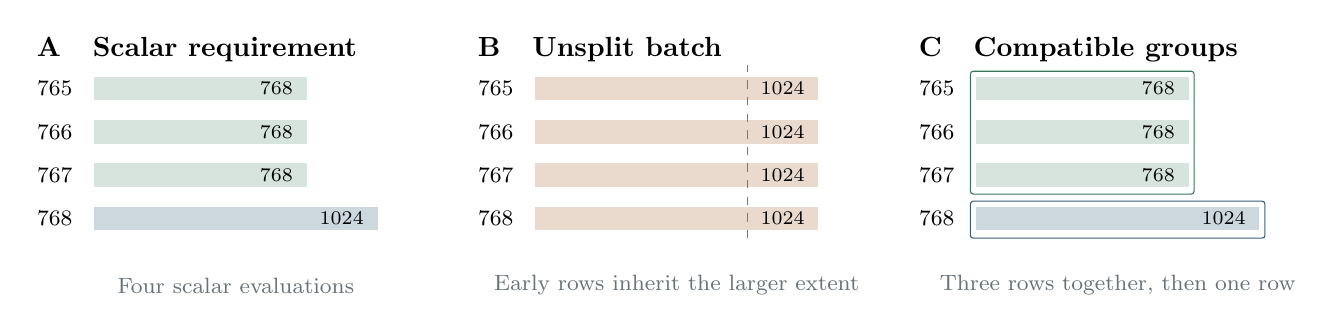
\begin{tikzpicture}[x=1cm,y=1cm,font=\small]
\node[anchor=west,font=\bfseries] at (0,2.9) {A\quad Scalar requirement};
\node[anchor=west,font=\bfseries] at (5.6,2.9) {B\quad Unsplit batch};
\node[anchor=west,font=\bfseries] at (11.2,2.9) {C\quad Compatible groups};
\foreach \row/\pos in {0/765,1/766,2/767,3/768}{
 \pgfmathsetmacro{\yy}{2.25-.55*\row}
 \node[anchor=east,font=\footnotesize] at (.7,\yy+.15) {\pos};
 \node[anchor=east,font=\footnotesize] at (6.3,\yy+.15) {\pos};
 \node[anchor=east,font=\footnotesize] at (11.9,\yy+.15) {\pos};
 \fill[qualified!20] (.85,\yy) rectangle (3.55,\yy+.3);
 \fill[draft!25] (6.45,\yy) rectangle (10.05,\yy+.3);
 \fill[qualified!20] (12.05,\yy) rectangle (14.75,\yy+.3);
 \ifnum\row=3
  \fill[target!25] (.85,\yy) rectangle (4.45,\yy+.3);
  \fill[target!25] (12.05,\yy) rectangle (15.65,\yy+.3);
  \node[anchor=east,font=\scriptsize] at (4.4,\yy+.15) {1024};
  \node[anchor=east,font=\scriptsize] at (15.6,\yy+.15) {1024};
 \else
  \node[anchor=east,font=\scriptsize] at (3.5,\yy+.15) {768};
  \node[anchor=east,font=\scriptsize] at (14.7,\yy+.15) {768};
 \fi
 \node[anchor=east,font=\scriptsize] at (10,\yy+.15) {1024};
}
\draw[draft,dashed] (9.15,.5)--(9.15,2.7);
\draw[qualified,rounded corners=1pt] (11.98,1.06) rectangle (14.82,2.62);
\draw[target,rounded corners=1pt] (11.98,.5) rectangle (15.72,.97);
\node[align=center,font=\footnotesize,text=aux] at (2.65,-.1) {Four scalar evaluations};
\node[align=center,font=\footnotesize,text=aux] at (8.25,-.1) {Early rows inherit the larger extent};
\node[align=center,font=\footnotesize,text=aux] at (13.85,-.1) {Three rows together, then one row};
\end{tikzpicture}

\caption{Physical-prefix grouping at the observed boundary. Logical query positions and causal masks remain fixed. The ordinary batch exposes all rows to physical extent 1024. The repaired graph uses the scalar extent for each maximal adjacent group: three queries at 768 and one at 1024. The rectangles depict operand extents, not probabilities or measured kernel time.}
\label{fig:prefix}
\end{figure*}

Vulkan independently reproduces the same extent pattern after its projection repair. Its crossed-extent AV intervention changes the actual dispatch between noncontiguous and contiguous matvec paths~\cite{b570llamarepair}. The common factor is the physical representation presented to the backend. The two implementations need not change the same kernel in the same way.

\subsection{Activation arithmetic and placement are separate factors}
\label{sec:arithmetic}
Vulkan's original Q8 projection path uses F32 activations for one row but Q8\_1 activation quantization for multiple rows. Keeping the weight file fixed therefore does not keep projection arithmetic fixed. Replays using real Q/K/V operands reproduce this distinction. A scoped precision policy routes the batched projection through an existing F32-activation path without changing the Q8 weights or serializing the projection~\cite{b570llamarepair}.

Projection repair alone restores the development endpoints but leaves 99 committed full-vector differences, beginning at output 29. Adding physical-prefix grouping removes those differences. Disabling the prefix component in the same binary restores the projection-only trajectory and its 99 differences; disabling the precision component restores endpoint failures. These reversals distinguish the two factors and show why successful endpoints alone were insufficient to locate the complete repair.

A distinct CUDA Qwen3-14B case demonstrates a placement requirement. With identical normalized K operands, the original single-row path places K RoPE on CPU while the multirow path places it on CUDA. Captured outputs differ in 851 of 1,024 F32 values. Eight exact-operand native replays reproduce the own-path and crossed-backend outcomes. A row-count-dependent offload preference at head-normalization scaling propagates to RoPE. The repair queries the original preference using a read-only single-row geometry descriptor, leaving the actual batched tensor and numerical libraries unchanged~\cite{rtxqwenrepair}.

These interventions motivate three concrete requirements: physical prefix, activation arithmetic and placement of the affected operator class. They do not imply that all operators share one universal signature. Each backend must map the requirements to a supported execution path.

\section{Reference-preserving query batching}
\label{sec:method}
\subsection{Extracting scalar physical extents}
For the supported dense single-stream cache, let $H$ be the first slot of the current contiguous append, $q$ the number of appended rows, $N$ the allocated cache capacity and $P$ the runtime padding unit. The frozen implementation uses $P=\max(n_{\mathrm{pad}},256)$. Query $i$ requires scalar physical extent
\begin{equation}
e_i=\min\!\left(N,\max\!\left(P,P\left\lceil
\frac{H+i+1}{P}\right\rceil\right)\right),\quad 0\leq i<q.
\label{eq:extent}
\end{equation}
The extractor reads actual slot placement and occupancy. It requires dense occupancy ending at $H+q$, one contiguous stream and ordered causal positions; it does not infer $H$ from a prompt's nominal length. Cache holes, sliding-window storage, unrelated streams or noncontiguous insertion do not satisfy this extractor's premises.

The physical extent differs from the number of unmasked logical keys. It controls tensor descriptors and backend dispatch even when the added probabilities are zero. Consequently, clipping the mask alone is insufficient: K, V and the probability operand must represent the corresponding physical prefix.

\subsection{Partitioning compatible queries}
In the evaluated implementations, arithmetic policy is fixed for each plan, so compatible rows share the required physical extent. The planner scans rows in logical order and emits maximal adjacent equal-extent groups. A varying per-row arithmetic policy would additionally require cuts where that policy changes. In the observed four-row example, the result is $(3,768)$ followed by $(1,1024)$. Most batches that stay within one padding interval remain one group.

\begin{proposition}[Minimum contiguous partition]
For $q>0$ rows with compatibility keys $\sigma_0,\ldots,\sigma_{q-1}$, the minimum number of contiguous groups whose keys are constant is
\begin{equation}
G_{\min}=1+\sum_{i=1}^{q-1}\mathbf{1}[\sigma_i\ne\sigma_{i-1}].
\label{eq:groups}
\end{equation}
Maximal adjacent equal-key groups attain this count.
\end{proposition}
\begin{proof}
Every adjacent key change requires a cut. Cutting exactly at those changes yields constant-key groups and introduces no other cut.
\end{proof}
For contiguous append, fixed arithmetic policy and $q\leq P$, Equation~\eqref{eq:extent} crosses at most one padding boundary, so at most two groups are needed. This is a property of the partition constraint. Numerical correspondence additionally depends on the lowering and arithmetic paths described below.

\subsection{Lowering a group through paired views}
Within a group, PQ constructs separate one-query attention subgraphs. QB expresses those query instances through a batch coordinate. After the native attention permutation, it views Q from $(d,q,h_Q,1)$ as $(d,1,h_Q,q)$ and transforms the mask from $(e,q,1,1)$ to $(e,1,1,q)$. If Q has base $b_Q$ and original strides $s_0,s_1,s_2,s_3$, then
\begin{align}
\operatorname{addr}_{\MQ}(v,i,a,0)&=b_Q+v s_0+i s_1+a s_2,\\
\operatorname{addr}_{\QB}(v,0,a,i)&=b_Q+v s_0+a s_2+i s_1.
\end{align}
The two descriptors select the same scalar. The mask retains the corresponding query stride and causal values. K and V share one sequence's storage across the new query coordinate; the original grouped-query head mapping is retained. Ordered output recombination restores the query/head arrangement expected by the output projection.

For a shortened group, the native graph creates Q, K, V and mask views with the group's extent. A strided shortened mask is materialized contiguously when the backend requires it. V's actual transposed or nontransposed representation determines which dimension is shortened. Output groups are concatenated in query order. Projection and feed-forward computation remain batched; grouping is local to attention.

In exact arithmetic, the address and head mappings compute the same attention values. In finite precision, the purpose of the one-query organization and extent constraint is to preserve the reference-sensitive backend path. The native comparisons test this requirement directly. Equal extents alone do not prove that an arbitrary batched operator is numerically equivalent.

\begin{table}[t]
\caption{Planner and lowering operations. The input contains graph/cache metadata and the selected reference policy, not an input ID or answer.}
\label{tab:algorithm}
\begin{tabularx}{\columnwidth}{@{}rY@{}}\toprule
1 & Read actual stream, cache occupancy, append slots, positions and padding.\\
2 & Derive the scalar extent of each row using Equation~\eqref{eq:extent}.\\
3 & Obtain the required activation and placement policies for the affected operator classes.\\
4 & Scan adjacent compatible rows and emit $(\mathrm{begin},\mathrm{width},\mathrm{extent})$ groups.\\
5 & Lower each group with native head mapping, paired Q/mask views and shared K/V.\\
6 & Restore query order and execute the unchanged commit/reconciliation transaction.\\
7 & Reuse a graph only when its geometry and active numerical policies match.\\\bottomrule
\end{tabularx}
\end{table}

\subsection{Arithmetic policy and graph identity}
The frozen CUDA and Vulkan implementations realize the same extent rule and partition independently. Their backend adaptations preserve the arithmetic paths required by the original reference. Vulkan marks the affected Q8 projections to retain F32 activations and preserves the noncontiguous AV evaluation path where required. CUDA's Qwen adaptation retains the scalar-path placement preference at the identified head-normalization boundary. The original reference and inactive draft path retain their own declared recipes.

The repair is phase scoped. Target prefill and target verification can contain multiple rows; the native target/draft ownership, pending-token handling, acceptance, correction and rollback remain unchanged. The selected phase is established before both observed and ordinary decoding paths. A diagnostic callback does not control whether repair executes.

Graph identity includes every policy that can change the generated graph: layout, physical-prefix vector and affected arithmetic/placement choices. Nominal tensor shapes alone are insufficient. The frozen native prefix implementations bind the extent vector to reuse and keep the other policies fixed within their contexts. The accompanying shared implementation factors out extent extraction and partitioning and adds an explicit policy key to graph reuse; its CPU and source-integration checks are reported in \ref{app:shared}.

\subsection{Implementation domain}
\label{sec:domain}
The measured prefix repair covers dense causal, single-sequence, non-flash attention with F16 KV, compatible Q/mask types, integral head mapping and up to four occupied query rows. Unsupported attention sinks, bias paths and MLA require their own lowering. The Vulkan port currently admits the tested 128-channel, 32-query-head/8-KV-head geometry; its source still contains these explicit guards. The shared planner removes duplication in extent extraction and grouping, but broader graph admission and automatic cross-family policy selection remain separate integration work. Table~\ref{tab:coverage} states which rules were actually exercised.

\section{Evaluation design}
\label{sec:evaluation}
\subsection{Systems and comparisons}
The new Llama experiments use Llama-3.1-8B-Instruct and Llama-3.2-1B-Instruct Q8 target/draft weights, F16 KV, context capacity 1024, non-flash attention, draft length $k=3$ and cap128/native EOG. CUDA runs on an RTX 5070 Ti Laptop GPU. Vulkan runs on Arc B570 with an i5-13400 and driver 32.0.101.9150. Its output-blind capacity admission selects GPU target and CPU draft before scientific forwards~\cite{rtxllamarepair,b570llamarepair}. Each backend preserves its own original UB1 reference. Their input panels and placements are distinct.

We distinguish three comparisons. $R$ defines the response to preserve. $M_L$ is ordinary target-only greedy execution under layout $L$; $C_L$ adds drafting to that same layout. PQ compares local one-query attention with QB's representation. The measurements include $R$, $M_{\PQ}$, $M_{\QB}$, two identical $C_{\PQ}$ controls and $C_{\QB}$. Target-only continuation consumes one pending token per decode; its target capacity of four also affects prefill.

\subsection{Mechanism, confirmation and timing}
Development starts from retained counterexamples. Same-state consumers, exact-operand replays and factor reversals identify the repairs before the new confirmation panels are selected. Each platform then freezes its candidate and independently selects 24 previously unseen natural inputs, balanced across code/math and short/long strata. The Vulkan panel uses 128--384 or 512--768 native prompt tokens. Input exclusions and exact selection rules are preserved with each platform's panel. The two panels are not one jointly sampled cross-platform cohort.

Each confirmation comprises 48 original-reference requests and 240 candidate requests, including observer controls. Complete endpoints and committed vocabulary vectors are checked against the original scalar execution; speculative transactions and corresponding PQ/QB rows are also compared. The tests preserve rejected rows and failures rather than selecting successful output fragments.

Each platform completes six Williams sessions over all 24 inputs and six labels: 864 measured requests and 864 immediately paired warmups. Fresh contexts are created within each paid request. The service window charges context creation, prefill, generation, draft/verification where enabled, reconciliation, synchronization and teardown. Model loading is outside this window and separately recorded. Heavy tracing is disabled for timing.

\subsection{Estimands}
For input $i$ and session $s$, define the paired control mean
\begin{equation}
\bar t_{is,\PQ}=\tfrac12(t_{is,C_{\PQ_A}}+t_{is,C_{\PQ_B}}).
\end{equation}
The speculative layout ratio is the geometric mean of $t_{is,C_{\QB}}/\bar t_{is,\PQ}$, with equal input and session log weights. Draft value is
\begin{equation}
D_L=\operatorname{GM}\!\left(t_{is,M_L}/t_{is,C_L}\right);
\quad D_L>1\ \text{favors drafting}.
\label{eq:draftvalue}
\end{equation}
For PQ, the denominator is the arithmetic control mean. The prospective practical layout screen requires a reduction larger than both 2\% and the largest symmetric input-aggregate A/A imbalance, with every session favoring QB. It is an engineering screen, not a significance test.

The target-only QB/PQ ratio is reconstructed after the experiment from the same complete blocks and weights. It is a descriptive comparison, not a replacement primary endpoint. No new timings are added to change a screen result. Earlier scope, operator and service campaigns retain their original panels, timers and estimators.

\section{Results}
\label{sec:results}
\subsection{Structural repair and unseen confirmation}
The CUDA prefix repair removes the known Llama reference failure; disabling it restores the two historical speculative-arm failures. On Vulkan, the combined precision and prefix repair removes both endpoint failures and the 99 latent committed-vector differences. The independent factor reversals recover their respective predecessor trajectories. The results identify a common grouping rule with a backend-specific arithmetic requirement.

All 24 confirmation inputs pass on each platform. Saved comparisons establish exact committed full-vocabulary vector correspondence with each original reference, in addition to endpoint agreement. The implementations were frozen before confirmation; each platform uses its own independently selected input panel.

\begin{table*}[t]
\centering\small
\caption{Numerical requirements exercised by each measured model/backend configuration.}
\label{tab:coverage}
\begin{tabularx}{\textwidth}{@{}>{\raggedright\arraybackslash}p{2.8cm}>{\raggedright\arraybackslash}p{3.7cm}Y@{}}\toprule
Model/backend & Active requirement and evidence & Interpretation\\\midrule
Llama Q8 / CUDA & Prefix grouping; known failure reversed; 24 unseen inputs & Active repair and input transfer on the frozen native implementation.\\
Llama Q8 / Vulkan & F32 activation path plus prefix grouping; independent reversals; 24 unseen inputs & Both factors are required for the observed numerical correspondence.\\
Qwen3-14B / CUDA & Scalar-path head-normalization placement; 12 unseen inputs in the earlier repair study & A second reference-sensitive operator mechanism, with successful targeted repair.\\
Qwen3-8B and 14B / CUDA & Combined build loads placement and prefix code; regression passes & Compatibility of the combined build; actual Qwen prefix-split activation is not established by these records.\\
Qwen3 / Vulkan & Historical layout adapter; new precision and prefix switches off & Old-path compatibility only; the new rules have not been actively transferred.\\
SmolLM2 / CUDA & Earlier PQ/QB and scope experiments & Supports the local layout comparison; not a regression of the new prefix/precision integration.\\\bottomrule
\end{tabularx}
\end{table*}

Table~\ref{tab:coverage} distinguishes active numerical repairs from compatibility regressions. The completed cross-backend result is the shared Llama physical-prefix rule; the Qwen placement result establishes a separate reference-sensitive operator requirement.

\subsection{Complete cost after Llama repair}
Table~\ref{tab:costs} reports all primary and descriptive ratios from the complete timing blocks. The two speculative layout reductions are 2.4469\% on CUDA and 4.9451\% on Vulkan. Every session favors QB. CUDA's reduction is below its 2.9832\% A/A screen; Vulkan exceeds its 2.9418\% screen, retaining the two slower blocks among all 144 blocks.

\begin{table*}[t]\centering\small
\caption{Reconstructed complete-request ratios on the two new Llama panels. Each platform uses all 144 paired blocks. The target-only layout comparison is post hoc; the practical screen applies to the speculative layout comparison.}
\label{tab:costs}
\begin{tabularx}{\textwidth}{@{}lrrY@{}}\toprule
Comparison & CUDA & Vulkan & Meaning\\\midrule
$C_{\QB}/\overline{C_{\PQ}}$ & 0.9755 & 0.9505 & Speculative layout; primary\\
$M_{\QB}/M_{\PQ}$ & 1.0044 & 0.8993 & Target-only layout; post hoc\\
$M_{\QB}/C_{\QB}$ & 0.9736 & 0.3343 & Draft value; above one favors draft\\
$C_{\QB}/R$ & 0.4590 & 1.6288 & Complete speculative path\\
$M_{\QB}/R$ & 0.4469 & 0.5444 & Complete target-only path\\
A/A screen & 2.983\% & 2.942\% & Predeclared engineering threshold\\
Speculative layout screen & Not passed & Passed & Requires all six sessions favorable\\
Slower speculative blocks & 38/144 & 2/144 & All blocks retained\\\bottomrule
\end{tabularx}\end{table*}


\begin{figure*}[t]\centering
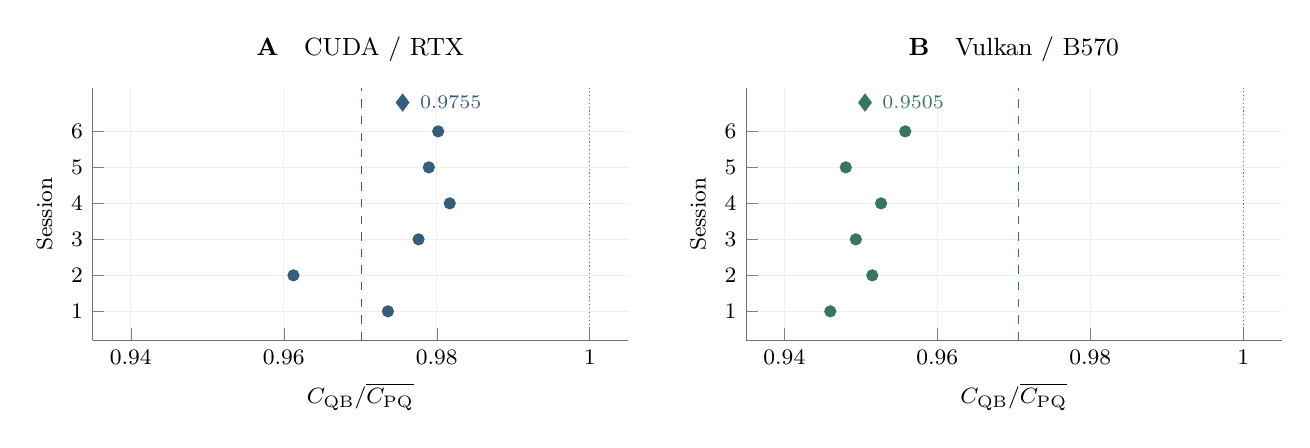
\begin{tikzpicture}
\begin{axis}[at={(0.6cm,0cm)},anchor=south west,scale only axis,
width=6.8cm,height=3.2cm,xmin=.935,xmax=1.005,ymin=.2,ymax=7.2,
ytick={1,2,3,4,5,6},yticklabels={1,2,3,4,5,6},
xtick={.94,.96,.98,1},xlabel={$C_{\QB}/\overline{C_{\PQ}}$},ylabel={Session},
title={\textbf{A}\quad CUDA / RTX},title style={font=\small},tick label style={font=\footnotesize},
label style={font=\footnotesize},grid=major,grid style={gray!13},
axis lines*=left,axis line style={aux},clip=false]
\addplot[aux,densely dotted,forget plot] coordinates {(1,.2)(1,7.2)};
\addplot[target,dashed,forget plot] coordinates {(0.970168433252,.2)(0.970168433252,7.2)};
\addplot[only marks,mark=*,mark size=2pt,target] coordinates {(0.973614560955,1) (0.961260204728,2) (0.977617954201,3) (0.981693410244,4) (0.978961967148,5) (0.980182883671,6)};
\addplot[only marks,mark=diamond*,mark size=3pt,target] coordinates {(0.975530832969,6.8)};
\node[font=\scriptsize,anchor=west,text=target] at (axis cs:0.976530832969,6.8) {0.9755};
\end{axis}
\begin{axis}[at={(8.9cm,0cm)},anchor=south west,scale only axis,
width=6.8cm,height=3.2cm,xmin=.935,xmax=1.005,ymin=.2,ymax=7.2,
ytick={1,2,3,4,5,6},yticklabels={1,2,3,4,5,6},
xtick={.94,.96,.98,1},xlabel={$C_{\QB}/\overline{C_{\PQ}}$},ylabel={Session},
title={\textbf{B}\quad Vulkan / B570},title style={font=\small},tick label style={font=\footnotesize},
label style={font=\footnotesize},grid=major,grid style={gray!13},
axis lines*=left,axis line style={aux},clip=false]
\addplot[aux,densely dotted,forget plot] coordinates {(1,.2)(1,7.2)};
\addplot[qualified,dashed,forget plot] coordinates {(0.970581674995,.2)(0.970581674995,7.2)};
\addplot[only marks,mark=*,mark size=2pt,qualified] coordinates {(0.946005141202,1) (0.951493999596,2) (0.949342846100,3) (0.952645421505,4) (0.948029478726,5) (0.955806566990,6)};
\addplot[only marks,mark=diamond*,mark size=3pt,qualified] coordinates {(0.950548530600,6.8)};
\node[font=\scriptsize,anchor=west,text=qualified] at (axis cs:0.951548530600,6.8) {0.9505};
\end{axis}
\end{tikzpicture}

\caption{Speculative QB versus the arithmetic pair of PQ controls on the two independently frozen Llama panels. Dots show all six session ratios; diamonds show the equal-weight aggregate. The dashed threshold is each study's predeclared practical screen, including A/A imbalance. Lower values favor QB. These are within-platform comparisons; the shared axis does not rank GPU speed.}
\label{fig:layoutcost}
\end{figure*}

Draft value is 0.9736 on CUDA and 0.3343 on Vulkan. Thus speculative QB costs about 1.027 and 2.992 times their respective target-only QB paths. The CPU-draft placement is part of the Vulkan execution, but no isolated placement intervention attributes the entire cost difference to it.

Target-only requests use multirow capacity during prefill and single-row autoregressive continuation. Their complete-request QB/PQ ratios are 1.0044 on CUDA and 0.8993 on Vulkan, corresponding to a 10.07\% Vulkan reduction. These post-hoc paired comparisons describe the combined prefill, generation and teardown cost. Relative to the original scalar recipes, $M_{\QB}/R$ is 0.4469 and 0.5444. Those savings include changes in prefill geometry and scoped arithmetic; the current service timer measures their combined effect.

\subsection{A second arithmetic mechanism: Qwen3-14B}
The earlier CUDA placement repair preserves all 12 preselected Qwen3-14B confirmation inputs against the original reference~\cite{rtxqwenrepair}. Its same-layout draft value is 1.4256, and complete $C_{\QB}/R$ is 0.3205 under the fixed partial-offload contract. The QB/PQ reduction is 2.61\%, below that campaign's 3.384\% practical screen. This supplies a positive drafting case alongside the new Llama results, under a different panel and placement. It also demonstrates why reference-compatible execution includes operator placement as well as attention representation.

\subsection{Repair scope and the local representation increment}
An earlier registered seven-arm study varies GS/PQ/QB and drafting on two fixed twelve-input panels over three dates~\cite{rtxscopetransfer}. Qwen3's draft value rises from 0.835 under global serialization to 1.122 under PQ and 1.188 under QB. SmolLM2 remains below parity at 0.684, 0.805 and 0.805. Each date preserves these draft decisions.

\begin{figure*}[t]\centering
\resizebox{\textwidth}{!}{% Generated from immutable session logs; ranges are observed date ranges.
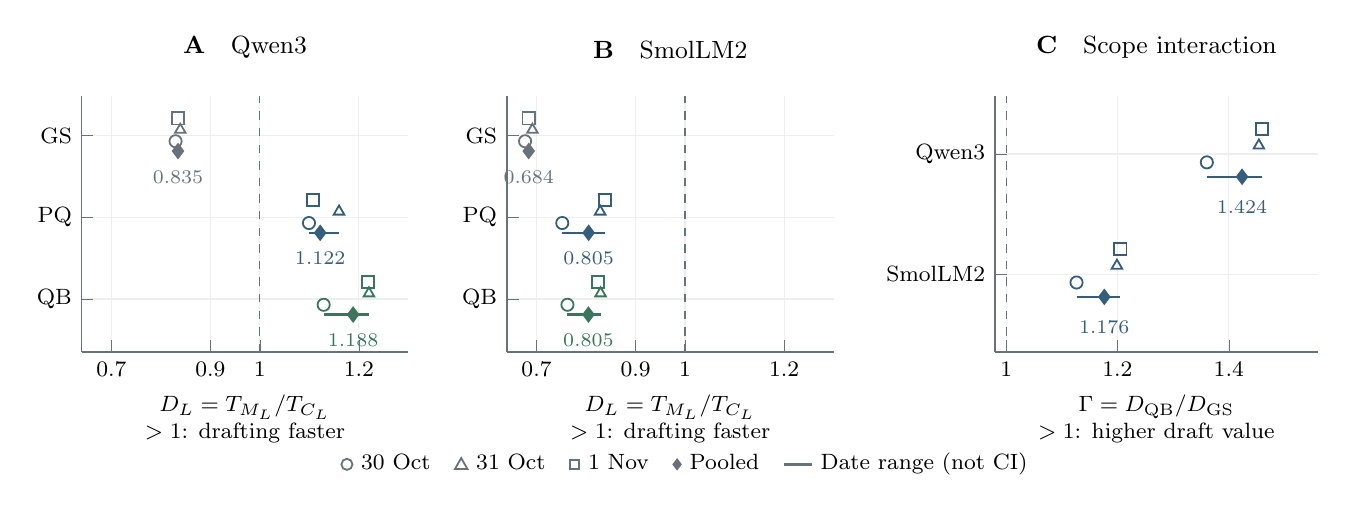
\begin{tikzpicture}
\begin{axis}[at={(0.6cm,0cm)},anchor=south west,scale only axis,
width=4.15cm,height=3.25cm,xmin=0.64,xmax=1.3,
ymin=.35,ymax=3.48,ytick={1,2,3},yticklabels={QB,PQ,GS},xtick={.7,.9,1,1.2},
axis lines*=left,axis line style={aux,line width=.5pt},tick style={aux},
tick label style={font=\footnotesize},grid=major,grid style={gray!13},
title={\textbf{A}\quad Qwen3},title style={font=\small,yshift=4pt},
xlabel={$D_L=T_{M_L}/T_{C_L}$\\$>1$: drafting faster},xlabel style={font=\footnotesize,align=center},clip=false]
\addplot[aux,dashed,forget plot] coordinates {(1,.35)(1,3.48)};
\addplot[aux,line width=.9pt,forget plot] coordinates {(0.829731004118,2.81)(0.839247877433,2.81)};
\addplot[only marks,mark=o,mark size=2.2pt,line width=.65pt,aux,forget plot] coordinates {(0.829731004118,2.93)};
\addplot[only marks,mark=triangle,mark size=2.2pt,line width=.65pt,aux,forget plot] coordinates {(0.839247877433,3.07)};
\addplot[only marks,mark=square,mark size=2.2pt,line width=.65pt,aux,forget plot] coordinates {(0.835003346314,3.21)};
\addplot[only marks,mark=diamond*,mark size=2.7pt,aux,forget plot] coordinates {(0.834651660975,2.81)};
\node[font=\scriptsize,text=aux,anchor=north] at (axis cs:0.834651660975,2.69){0.835};
\addplot[target,line width=.9pt,forget plot] coordinates {(1.099220287892,1.81)(1.159930527291,1.81)};
\addplot[only marks,mark=o,mark size=2.2pt,line width=.65pt,target,forget plot] coordinates {(1.099220287892,1.93)};
\addplot[only marks,mark=triangle,mark size=2.2pt,line width=.65pt,target,forget plot] coordinates {(1.159930527291,2.07)};
\addplot[only marks,mark=square,mark size=2.2pt,line width=.65pt,target,forget plot] coordinates {(1.107396324397,2.21)};
\addplot[only marks,mark=diamond*,mark size=2.7pt,target,forget plot] coordinates {(1.121863272924,1.81)};
\node[font=\scriptsize,text=target,anchor=north] at (axis cs:1.121863272924,1.69){1.122};
\addplot[qualified,line width=.9pt,forget plot] coordinates {(1.128912764045,0.81)(1.220335090837,0.81)};
\addplot[only marks,mark=o,mark size=2.2pt,line width=.65pt,qualified,forget plot] coordinates {(1.128912764045,0.93)};
\addplot[only marks,mark=triangle,mark size=2.2pt,line width=.65pt,qualified,forget plot] coordinates {(1.220335090837,1.07)};
\addplot[only marks,mark=square,mark size=2.2pt,line width=.65pt,qualified,forget plot] coordinates {(1.218401922887,1.21)};
\addplot[only marks,mark=diamond*,mark size=2.7pt,qualified,forget plot] coordinates {(1.188438428122,0.81)};
\node[font=\scriptsize,text=qualified,anchor=north] at (axis cs:1.188438428122,0.69){1.188};
\end{axis}
\begin{axis}[at={(6.0cm,0cm)},anchor=south west,scale only axis,
width=4.15cm,height=3.25cm,xmin=0.64,xmax=1.3,
ymin=.35,ymax=3.48,ytick={1,2,3},yticklabels={QB,PQ,GS},xtick={.7,.9,1,1.2},
axis lines*=left,axis line style={aux,line width=.5pt},tick style={aux},
tick label style={font=\footnotesize},grid=major,grid style={gray!13},
title={\textbf{B}\quad SmolLM2},title style={font=\small,yshift=4pt},
xlabel={$D_L=T_{M_L}/T_{C_L}$\\$>1$: drafting faster},xlabel style={font=\footnotesize,align=center},clip=false]
\addplot[aux,dashed,forget plot] coordinates {(1,.35)(1,3.48)};
\addplot[aux,line width=.9pt,forget plot] coordinates {(0.676863315065,2.81)(0.691715651785,2.81)};
\addplot[only marks,mark=o,mark size=2.2pt,line width=.65pt,aux,forget plot] coordinates {(0.676863315065,2.93)};
\addplot[only marks,mark=triangle,mark size=2.2pt,line width=.65pt,aux,forget plot] coordinates {(0.691715651785,3.07)};
\addplot[only marks,mark=square,mark size=2.2pt,line width=.65pt,aux,forget plot] coordinates {(0.684117166690,3.21)};
\addplot[only marks,mark=diamond*,mark size=2.7pt,aux,forget plot] coordinates {(0.684205177029,2.81)};
\node[font=\scriptsize,text=aux,anchor=north] at (axis cs:0.684205177029,2.69){0.684};
\addplot[target,line width=.9pt,forget plot] coordinates {(0.751980461104,1.81)(0.838157410742,1.81)};
\addplot[only marks,mark=o,mark size=2.2pt,line width=.65pt,target,forget plot] coordinates {(0.751980461104,1.93)};
\addplot[only marks,mark=triangle,mark size=2.2pt,line width=.65pt,target,forget plot] coordinates {(0.828542225334,2.07)};
\addplot[only marks,mark=square,mark size=2.2pt,line width=.65pt,target,forget plot] coordinates {(0.838157410742,2.21)};
\addplot[only marks,mark=diamond*,mark size=2.7pt,target,forget plot] coordinates {(0.805283741164,1.81)};
\node[font=\scriptsize,text=target,anchor=north] at (axis cs:0.805283741164,1.69){0.805};
\addplot[qualified,line width=.9pt,forget plot] coordinates {(0.762480613719,0.81)(0.829418625217,0.81)};
\addplot[only marks,mark=o,mark size=2.2pt,line width=.65pt,qualified,forget plot] coordinates {(0.762480613719,0.93)};
\addplot[only marks,mark=triangle,mark size=2.2pt,line width=.65pt,qualified,forget plot] coordinates {(0.829418625217,1.07)};
\addplot[only marks,mark=square,mark size=2.2pt,line width=.65pt,qualified,forget plot] coordinates {(0.824490025340,1.21)};
\addplot[only marks,mark=diamond*,mark size=2.7pt,qualified,forget plot] coordinates {(0.804876656398,0.81)};
\node[font=\scriptsize,text=qualified,anchor=north] at (axis cs:0.804876656398,0.69){0.805};
\end{axis}
\begin{axis}[at={(12.2cm,0cm)},anchor=south west,scale only axis,
width=4.1cm,height=3.25cm,xmin=0.98,xmax=1.56,
ymin=.35,ymax=2.48,ytick={1,2},yticklabels={SmolLM2,Qwen3},xtick={1,1.2,1.4},
axis lines*=left,axis line style={aux,line width=.5pt},tick style={aux},
tick label style={font=\footnotesize},grid=major,grid style={gray!13},
title={\textbf{C}\quad Scope interaction},title style={font=\small,yshift=4pt},
xlabel={$\Gamma=D_{\QB}/D_{\GS}$\\$>1$: higher draft value},xlabel style={font=\footnotesize,align=center},clip=false]
\addplot[aux,dashed,forget plot] coordinates {(1,.35)(1,2.48)};
\addplot[target,line width=.9pt,forget plot] coordinates {(1.360576811570,1.81)(1.459158131838,1.81)};
\addplot[only marks,mark=o,mark size=2.2pt,line width=.65pt,target,forget plot] coordinates {(1.360576811570,1.93)};
\addplot[only marks,mark=triangle,mark size=2.2pt,line width=.65pt,target,forget plot] coordinates {(1.454081831663,2.07)};
\addplot[only marks,mark=square,mark size=2.2pt,line width=.65pt,target,forget plot] coordinates {(1.459158131838,2.21)};
\addplot[only marks,mark=diamond*,mark size=2.7pt,target,forget plot] coordinates {(1.423873555506,1.81)};
\node[font=\scriptsize,text=target,anchor=north] at (axis cs:1.423873555506,1.69){1.424};
\addplot[target,line width=.9pt,forget plot] coordinates {(1.126491267510,0.81)(1.205188329550,0.81)};
\addplot[only marks,mark=o,mark size=2.2pt,line width=.65pt,target,forget plot] coordinates {(1.126491267510,0.93)};
\addplot[only marks,mark=triangle,mark size=2.2pt,line width=.65pt,target,forget plot] coordinates {(1.199074537459,1.07)};
\addplot[only marks,mark=square,mark size=2.2pt,line width=.65pt,target,forget plot] coordinates {(1.205188329550,1.21)};
\addplot[only marks,mark=diamond*,mark size=2.7pt,target,forget plot] coordinates {(1.176367387182,0.81)};
\node[font=\scriptsize,text=target,anchor=north] at (axis cs:1.176367387182,0.69){1.176};
\end{axis}
\node[anchor=north,font=\footnotesize] at (8.25,-1.15) {\tikz[baseline=-.5ex]\draw[aux,line width=.65pt] (0,0) circle (2pt);\ 30 Oct\quad \tikz[baseline=-.5ex]\draw[aux,line width=.65pt] (0,.08)--(.08,-.06)--(-.08,-.06)--cycle;\ 31 Oct\quad \tikz[baseline=-.5ex]\draw[aux,line width=.65pt] (-.06,-.06) rectangle (.06,.06);\ 1 Nov\quad \tikz[baseline=-.5ex]\fill[aux] (0,.08)--(.06,0)--(0,-.08)--(-.06,0)--cycle;\ Pooled\quad \tikz[baseline=-.5ex]\draw[aux,line width=.9pt] (0,0)--(.35,0);\ Date range (not CI)};
\end{tikzpicture}

}
\caption{Earlier repair-scope study, retained under its original panel and resident-service window. $D_L>1$ favors drafting. Open symbols are the three actual date means; diamonds pool them with equal log weights. The line spans observed date values, not a confidence interval. Qwen3 benefits from drafting under local repair; SmolLM2 does not.}
\label{fig:scope}
\end{figure*}

The same-panel scope interaction factors as
\begin{equation}
\frac{D_{\QB}}{D_{\GS}}
=\frac{D_{\PQ}}{D_{\GS}}\,
\frac{D_{\QB}}{D_{\PQ}}.
\end{equation}
The factors are $1.3441\times1.0593$ for Qwen3 and $1.1770\times0.9995$ for SmolLM2. This separates the change from global to local repair from QB's incremental representation effect. Recorded logical work is matched across Qwen3 scopes; SmolLM2's work changes, making its result a joint request-path effect.

Separate three-family local-layout measurements find 2.83--6.17\% lower speculative request latency for QB than PQ, and 72 real attention contexts establish bitwise PQ/QB stage correspondence~\cite{studyrecords}. A matched Qwen3 study retains the $k=3$ layout benefit with resident and fresh contexts, at 6.26\% and 5.36\%; neither $k=1$ cell passes its practical screen~\cite{rtxnativebridge}. These measurements motivate retaining QB inside compatible groups. Their short-context correspondence does not replace the later physical-prefix repair.

\subsection{State as a requirement on composition}
The earlier Vulkan producer--consumer study establishes a state-composition effect~\cite{b570producer}. On two of eight inputs, changing the producer state switches PQ/QB from divergence to preservation while both natural serial continuations retain the same original reference. All sixteen input--producer pairs preserve PQ/QB agreement. The input state therefore affects whether local correspondence composes with the reference.

The Llama repairs connect this state-composition concern to concrete activation and attention operations. The Qwen producer-state cases retain their original status: the new Vulkan policies were inactive in their regression.

\section{Related work and application scope}
\label{sec:related}
Batch-invariant inference already identifies batch-dependent reduction choices in normalization, matrix multiplication and attention~\cite{thinkingmachines}. Its attention discussion includes query length, KV layout and fixed split-size evaluation. HeteroSpec identifies which physical execution conditions must be retained for a pre-existing quantized reference and realizes them through local grouping and backend arithmetic policies.

CoRun establishes deterministic execution using isolated prefill and fixed-shape batched decode~\cite{corun}. LLM-42 reuses shape-consistent kernels in a fast-path/verify--rollback design~\cite{llm42}. The verifier supplies the consistent numerical execution, and successful token verification still replaces KV entries with verified state. HeteroSpec constrains the optimized path to the original scalar deployment and adds no separate online consistency verifier.

Vosti connects a canonical prefix state to relational kernel contracts and an inductive engine proof~\cite{vosti}. Its kernel-contract documentation explicitly distinguishes this system-level determinism from numerical equivalence to an existing reference implementation~\cite{vosticontract}. Compatibility with the established execution is the central objective here.

Query parallelism itself is established attention structure. FlashAttention and FlashAttention-2 use tiling and query-row work partitioning to improve fused attention~\cite{flashattention,flashattention2}. QB uses views of existing non-flash operators to retain a local one-query organization. LayerCast changes computation precision while retaining lower-precision weight storage~\cite{layercast}; our Vulkan precision policy specifically matches the original path's activation handling. State-transplantation and cache-induced divergence studies motivate examining the producer state~\cite{stagereplay,cachestate}. The contribution here is the transition from a state-dependent failure to controlled operator interventions and a structural repair.

\paragraph{Application scope}
The target setting is a quantized deployment whose established numerical behavior must remain compatible while prompt or speculative-verification work is batched. The evidence covers the configurations in Table~\ref{tab:coverage}, single-stream non-flash attention and context capacity 1024. The strongest completed transfer is a common physical-prefix rule across two backend implementations, followed by independent unseen-input confirmation. Active cross-family policy extraction, wider cache organizations and concurrent serving are extensions of this implementation.

\section{Conclusion}
HeteroSpec organizes available query parallelism around the execution requirements of an existing numerical reference. Physical-prefix grouping repairs a common CUDA/Vulkan attention failure; matching activation arithmetic and operator placement addresses separate backend-sensitive paths. Paired query/mask views retain parallel work inside compatible groups.

Native interventions, factor reversals and two independent unseen-input panels establish the completed Llama repair. Complete-request comparisons show the distinct roles of reference compatibility, local layout cost and drafting: Vulkan's repaired QB path improves over PQ, while the same-layout target-only paths remain preferable for the new Llama workloads. The resulting design principle is concrete: preserve reference-sensitive execution dimensions and batch along the independent dimensions that remain.

\section*{Data and code availability}
Commit-pinned native implementations, input identities, full-vector records and request measurements are indexed in \ref{app:artifacts}. This source package includes the reported timing records, their reconstruction script and editable figures. The companion shared planner and native adapters are supplied as a separately identified integration candidate; all GPU results in this paper come from the frozen implementations identified in the tables.
\section*{Declaration of AI-assisted work}
OpenAI ChatGPT and Codex assisted implementation, analysis code, figures and writing. Scientific Agent Skills supported the developmental review~\cite{scientificskills}. Measurements come from recorded native executions. The author is responsible for verifying the results, interpretations and references and approving the final text.
\bibliographystyle{psql-num}
\balance
\bibliography{references}
\clearpage
\appendix
\section{Numerical and transactional conditions}
\label{app:conditions}
The runtime preserves the reference through both computation and state ownership. Each target cycle consumes the pending token exactly once, verifies the supplied draft rows, commits accepted tokens and a correction or bonus as appropriate, and removes rejected KV positions before continuing. A reference-preserving attention call cannot compensate for a different state supplied upstream. The observed producer effects and the Vulkan activation intervention motivate checking that state as well as local operators.

QB preserves the native head map $\kappa(a)$ and query order. For query $i$ and head $a$, QK selects the same Q and K entries, softmax uses the corresponding causal mask, and AV reads the same visible V values. Physical-prefix grouping additionally preserves the descriptor extent used for the scalar query. The backend adapter must retain the applicable arithmetic path. This decomposition explains which observations support which part of the implementation: address checks establish indexing, native stage comparisons establish the captured numerical behavior, and complete requests test their stateful composition.

The source guards are executable conditions, not a classifier predicting arbitrary future input behavior. No online execution of $R$ is charged or used to select a path in the reported timings. The method's finite confirmation applies to its frozen configuration and output window. The existing diagnostic fallback for unsupported graph features is not relabeled as a universal reference guarantee.

\section{Evidence and model-transfer details}
\label{app:transfer}
The original CUDA Llama diagnostic contains 54 requests and 5,916 complete vectors. Its natural failure is at output 81; mapping saved vectors reveals the earlier common-prefix discrepancy at output 29. The causal study uses same-state consumers and crossed physical extents. Late-cycle consumers can already agree on a wrong original-reference decision because earlier state differences have propagated.

Vulkan recovers that diagnostic before its independent development. Its projection-only candidate passes development endpoints but retains 99 committed vector differences. The combined development matrix contains 36 requests, 3,152 saved vectors and 1,920 committed candidate vectors. Disabling prefix grouping restores the projection-only matrix; disabling Q8 precision control restores endpoint failures. The stock reference remains unchanged. These factor reversals support the two-mechanism interpretation.

The CUDA Qwen3-14B placement repair has a separate twelve-input unseen confirmation. In the later combined-build regressions, Qwen3-8B uses twelve exposed inputs and Qwen3-14B uses sixteen, with 144/192 candidate requests and 24/32 original-reference requests. Both placement and prefix code are loaded. The summaries do not independently count actual prefix-split events, so these results establish combined-build compatibility.

Vulkan's historical Qwen adapter sets the layout but leaves the new precision and prefix switches off. Its twelve-request regression and 914 saved vectors/descriptors establish compatibility of the prior path. The two original P1 consumer failures on MATH-500 prealgebra/1865 and /1804 therefore remain active transfer targets. Their P4T consumer paths already pass, so switching the producer to P4T would not demonstrate that the new rule repairs P1. GSM8K/train/1184 additionally changes the natural serial endpoint under P4T and tests the producer side.

RTX's extra non-reference committed-vector comparison is a descriptive reconstruction beyond its registered endpoint/observer gates; it is not a newly imposed prospective gate. Both platforms' saved comparisons include candidate-R controls. No model forward was run for this manuscript revision.

The CUDA confirmation audit reconstructs 23,080 saved vectors; its 120 committed-vector comparison items contain no differences from the original reference. Vulkan reconstructs 23,718 saved vectors and compares 14,555 committed candidate vectors exactly with the original scalar vectors. These totals describe saved checks; the experimental unit remains the input.

\section{Complete-cost reconstruction}
\label{app:cost}
The source package retains all 144 blocks per platform, each with six measured service times. The reconstruction uses the stored values directly; it recomputes arithmetic PQ controls, session means, equal-weight log aggregates, A/A screens and slower-block counts. All 1,728 measured times are included. Warmup completion and native endpoint checks remain in the source-host audit.

On CUDA, 38 of 144 speculative QB blocks are slower than the PQ control mean; on Vulkan, two are slower. For target-only QB/PQ, the counts are 73 and zero. Thus a favorable session aggregate is not equivalent to every individual request improving. The target-only ratio is a post-hoc paired description.

The observed six-session speculative ratios are
\[
\begin{array}{ll}
\text{CUDA:}&.97361,\ .96126,\ .97762,\\
           &.98169,\ .97896,\ .98018;\\[2pt]
\text{Vulkan:}&.94601,\ .95149,\ .94934,\\
             &.95265,\ .94803,\ .95581.
\end{array}
\]
The screening thresholds are computed from the original input-aggregate symmetric A/A definition. The practical screen is not an interval estimate of a population effect. No pooling combines the two devices or the earlier twelve-input studies.

The target-only loop still decodes one pending token per iteration. Its UB4 capacity permits multirow prefill. Consequently, $M_{\QB}/R$ combines prefill geometry, scoped arithmetic and complete-path costs. The present time window supports the total comparison; a dedicated stage diagnostic is needed to assign a contribution to prefill. All arms load their declared model resources outside the service window, while target-only generation creates no draft context and performs no draft computation.

Earlier experiments retain useful independent roles: the three-family E1/E2 study tests local PQ/QB correspondence and representation cost; the matched Qwen3 lifecycle study tests $k$ and context lifetime; the three-date GS/PQ/QB study tests scope and draft value; the Vulkan state study supplies producer-dependent counterexamples. Their complete records remain in the earlier source package~\cite{paperbaseline}. They are not converted into new Llama replicates.

\section{Shared source implementation}
\label{app:shared}
The shared C++17 planner accepts actual cache occupancy, append slots, capacity and padding. It returns scalar extents and a maximal adjacent partition, using wide intermediate arithmetic for padding. The native integration script replaces the duplicate extractor and grouping code in recovered CUDA/Vulkan source trees and includes explicit policy identity in the graph reuse predicate. It writes a separate candidate tree and preserves the source guards.

CPU validation compares extents with an independently implemented scalar-allocation loop, covers padding boundaries and capacity limits, checks rejected sparse/noncontiguous states, and compares small partitions with exhaustive contiguous alternatives. Integration checks compile the generated cache method and reject source drift. The policy-key checks distinguish same-shaped graphs with different layout, precision, prefix and head-normalization choices.

This revision's native integration uses the shared prefix planner. The arithmetic/dispatch requirement interface is not yet connected to an automatic backend extractor. GPU results remain attributed to the frozen native implementations, not the refactored candidate.

\section{Artifact entrypoints and access}
\label{app:artifacts}
The manuscript uses the following fixed evidence snapshots:
\begin{itemize}[itemsep=2pt]
\item CUDA Llama: PR162, \texttt{e11d2b75}, with scientific execution snapshot \texttt{70086c63}; \path{benchmarks/rtx_llama_repair_v1/host_execution/}.
\item Vulkan Llama: PR163, \texttt{10a70566}; \path{benchmarks/b570_llama_companion_v1/host_execution/}.
\item CUDA Qwen3-14B repair: PR159, \texttt{38b3d3d3}; its result and addendum preserve the original PR156 reference.
\item Prior manuscript and analyses: PR154, \texttt{07bee1c5}, including the PR151 scope results and PR152 producer-state results.
\end{itemize}
Exact paths and Git blob identities for the files read during this revision accompany the source index. The paper's timing table and figure are generated by \texttt{scripts/reconstruct.py}; the inputs are \texttt{data/rtx\_cost.json} and \texttt{data/b570\_cost.json}. This is reconstruction from saved reports, not re-execution of raw model requests.

At the inspected heads, Vulkan's remote readback and restored scientific reconstruction are complete. CUDA's scientific execution and local reconstruction are complete, while its final remote delivery receipt remains in progress. Same-host reconstruction is distinct from independent-laboratory reproduction. Model weights remain externally acquired, pinned inputs. The repository and bulk artifacts require authorized access; publication access must be arranged before external review.

\end{document}
